\chapter{Analisis}
\label{chap:analisis}

\section{Analisis Permainan \textit{Snake} yang Sudah Ada}
Permainan \textit{Snake} yang akan dianalisis adalah \textit{Slither.io} dan \textit{Snake} pada telepon genggam \textit{Nokia}. \textit{Slither.io} adalah permainan \textit{web} yang dapat dimainkan oleh lebih dari 1 pemain(\textit{multiplayer}). Cara bermainya mirip seperti permainan \textit{Snake} pada umumnya yaitu ular harus memakan makanan untuk mendapatkan skor. Dalam permainan ini, setiap pemain berkompetisi untuk menjadi pemain terbaik dengan cara mendapatkan skor sebanyak-banyaknya. Pemain akan kalah apabila ular milik pemain menabrak ular milik pemain lain.\\

\textit{Snake} pada telepon genggam \textit{Nokia} hanya dapat dimainkan oleh 1 pemain. Dalam permainan ini, ular harus mendapatkan skor sebanyak-banyaknya dengan memakan makanan. Setiap memakan makanan, skor akan bertambah sebanyak 1 poin. Pemain akan kalah apabila ular menabrak dinding labirin dan menabrak tubuh sendiri.

\subsection{Ular dan Makanan}
Ular pada \textit{Slither.io} dibentuk dengan menggunakan sekumpulan lingkaran yang saling berdempetan satu sama lain seperti pada Gambar~\ref{fig:slitherUlar}. Bagian kepala pada ular ditandai menggunakan sepasang mata. Ketika memakan makanan, tubuh ular akan memanjang dengan menambahkan sebuah lingkaran pada bagian ekor ular. Setiap memulai permainan, tubuh ular akan memiliki warna yang ditentukan secara acak.\\

Makanan pada \textit{Slither.io} berbentuk lingkaran. Makanan ini ada yang berukuran besar dan ada yang berukuran kecil. Makanan ini tersebar pada labirin, jumlahnya sangat banyak dan warnanya bermacam-macam. Gambar~\ref{fig:slitherMakanan} merupakan sekumpulan makanan yang terdapat pada labirin. Setiap makanan akan menambah skor sebanyak 1 poin.

\begin{figure}[H]
	\centering  
	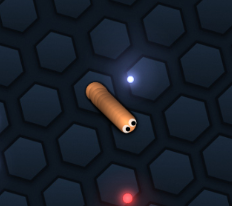
\includegraphics[scale=0.7]{slitherUlar}  
	\caption[Ular pada \textit{Silther.io}]{Ular pada \textit{Silther.io}}
	\label{fig:slitherUlar} 
\end{figure}

\begin{figure}[H]
	\centering  
	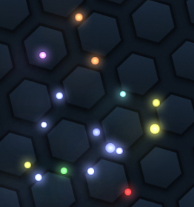
\includegraphics[scale=0.7]{slitherMakanan}  
	\caption[Makanan pada \textit{Slither.io}]{Makanan pada \textit{Slither.io}}
	\label{fig:slitherMakanan} 
\end{figure}

Ular pada \textit{Snake Nokia} dibuat seperti permainan 8 bit yang terdiri dari \textit{pixel-pixel} seperti pada Gambar~\ref{fig:snakeNokia}. Pada permainan ini apabila kepala ular sudah dekat dengan makanan, maka kepala ular akan terlihat sedang membuka mulutnya. Makanan yang terdapat pada permainan ini ada 2 macam yaitu makanan biasa dan makanan bonus seperti yang terlihat pada Gambar~\ref{fig:snakeFood}. Makanan biasa memiliki skor 1 poin dan makanan bonus memiliki skor 10 poin. Makanan bonus muncul secara acak dan memiliki batas waktu untuk berada pada labirin. Makanan bonus tidak hanya menambah skor lebih banyak tetapi makanan ini dapat membuat tubuh ular lebih panjang dibandingkan dengan memakan makanan biasa.

\begin{figure}[H]
	\centering  
	
\includegraphics[scale=1]{snakeNokia}  
	\caption[Ular pada \textit{Snake Nokia}]{Ular pada \textit{Snake Nokia}}
	\label{fig:snakeNokia} 
\end{figure}

\begin{figure}[H]
	\centering  
	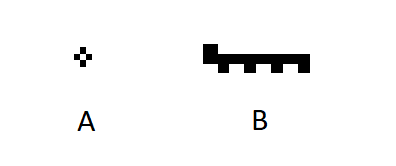
\includegraphics[scale=0.7]{snakeFood}  
	\caption[Makanan biasa(A) dan makanan bonus(B) pada \textit{Snake Nokia}]{Makanan biasa(A) dan makanan bonus(B) pada \textit{Snake Nokia}}
	\label{fig:snakeFood} 
\end{figure}

\subsection{Pergerakan Ular}
Ular pada \textit{Slither.io} digerakan dengan menggunakan \textit{keyboard} dan \textit{mouse}. Tombol ke kiri akan membuat ular bergerak berlawanan arah jarum jam dan tombol ke kanan akan membuat ular bergerak searah jarum jam. Semakin lama tombol ditekan, maka ular akan berbelok lebih cepat. Kursor pada \textit{mouse} membuat ular bergerak ke arah posisi kursor tersebut. Ular dapat melaju dengan cepat(\textit{speed up}) dengan menekan tombol \textit{mouse} kiri seperti yang terdapat pada Gambar~\ref{fig:slitherSpeed}. Ketika ular sedang melaju dengan cepat, total skor yang didapat akan berkurang. 

\begin{figure}[H]
	\centering  
	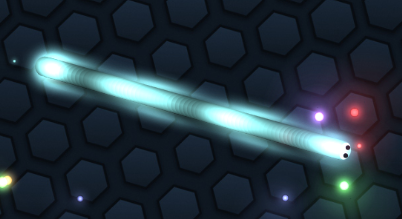
\includegraphics[scale=0.7]{slitherSpeed}  
	\caption[Ular sedang melaju dengan cepat(\textit{speed up})]{Ular sedang melaju dengan cepat(\textit{speed up})}
	\label{fig:slitherSpeed} 
\end{figure}

Ular pada \textit{Snake Nokia} hanya dapat bergerak ke atas, ke bawah, ke kiri dan ke kanan. Ular dapat digerakan menggunakan tombol angka pada telepon genggam Nokia yaitu tombol 8 untuk bergerak ke atas, tombol 4 untuk bergerak ke kiri, tombol 6 untuk bergerak ke kanan dan tombol 2 untuk bergerak ke bawah. Kecepatan ular juga dapat dipilih. Semakin tinggi tingkat, maka ular akan bergerak semakin cepat.

\subsection{Labirin}
Labirin pada \textit{Slither.io} hanya ada 1 saja. Labirin ini berbentuk lingkaran yang sisinya merupakan dinding. Apabila ular menabrak dinding labirin, maka permainan akan berakhir. Labirin ini cukup besar sehingga sangat kecil kemungkinan ular untuk menabrak dinding labirin. Gambar~\ref{fig:slitherLabirin} menunjukan peta labirin pada \textit{Slither.io}. Pada peta labirin tersebut terdapat sekumpulan titik bewarna abu-abu yang merepresentasikan makanan.

\begin{figure}[H]
	\centering  
	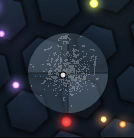
\includegraphics[scale=1]{slitherLabirin}  
	\caption[Peta labirin pada \textit{Slither.io}]{Peta labirin pada \textit{Slither.io}}
	\label{fig:slitherLabirin} 
\end{figure}

Labirin pada \textit{Snake Nokia} lebih bervariasi dibandingkan dengan \textit{Slither.io}. Pada permainan ini pemain dapat memilih labirin yang tersedia. Semakin tinggi level, maka labirin akan semakin rumit. 

\section{Analisis Sistem yang Dibangun}
Open Source Snake 360 memiliki cara bermain yang mirip seperti permainan Snake pada umumnya. Perbedaan antara Open Source Snake 360 dengan permainan \textit{Snake} pada umumnya adalah Open Source Snake 360 dapat menambahkan labirin sendiri. 

\subsection{Menggambar Ular dan Apel}
Tubuh ular dibuat menggunakan sekumpulan \textit{line}/garis pendek. Setiap bagian tubuh ular memiliki panjang sebesar 2 \textit{pixel} dan lebar tubuhnya sebesar 10 \textit{pixel}. Panjang setiap bagian tubuh ular tidak 1 pixel karena akan membuat ular terlihat sangat pendek. Bagian tubuh ular dibuat pendek untuk memudahkan pengecekan jika terjadi ular menabrak tubuhnya sendiri. Setiap bagian tubuh ular memiliki koordinat masing-masing. Koordinat setiap bagian tubuh disimpan pada sebuah \textit{array} agar menggambar ular menjadi lebih mudah. Dalam tahap ini, tubuh ular masih berupa sekumpulan titik-titik yang merupakan koordinat bagian tubuh ular seperti pada Gambar~\ref{fig:titikUlar}. Algoritma untuk menggambar ular adalah dengan mengambil koordinat bagian tubuh ular mulai dari elemen \textit{array} paling pertama(arr[0]) dan elemen \textit{array} selanjutnya(arr[1]) lalu buat garis yang \textit{start point}nya adalah elemen pertama(arr[0]) dan \textit{end point}nya adalah elemen \textit{array} kedua(arr[1]). Setelah itu ambil koordinat elemen \textit{array} yang merupakan \textit{end point} pada garis sebelumnya(arr[1]) dengan elemen \textit{array} selanjutnya(arr[2]) dan gambar garisnya. Lakukan hal tersebut sampai \textit{end point} garis mencapai elemen \textit{array} paling akhir. Setelah digambar maka ular akan terlihat seperti Gambar~\ref{fig:garisUlar}.

\begin{figure}[H]
	\centering  
	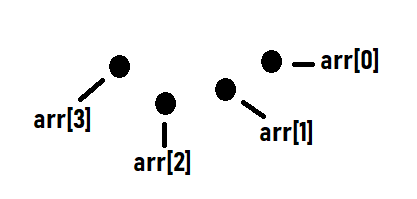
\includegraphics[scale=0.7]{titikUlar}  
	\caption[Koordinat bagian tubuh ular pada \textit{array}]{Koordinat bagian tubuh ular pada \textit{array}}
	\label{fig:titikUlar} 
\end{figure}

\begin{figure}[H]
	\centering  
	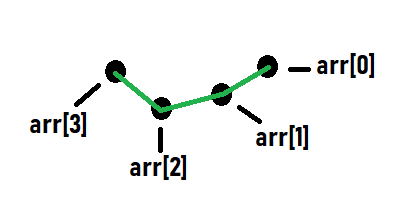
\includegraphics[scale=0.7]{garisUlar}  
	\caption[Tubuh ular setelah digambar menggunakan garis]{Tubuh ular setelah digambar menggunakan garis}
	\label{fig:garisUlar} 
\end{figure}

Untuk membuat apel digunakan \textit{quadratic B\'ezier curve}. Kurva ini digunakan untuk membuat bagian-bagian apel yang melengkung. Bagian tersebut ditandai dengan lingkaran bewarna merah seperti yang ditunjukan pada Gambar~\ref{fig:apel}(gambar diambil dari pinterest. Link:\url{https://www.pinterest.com/pin/690317449105509454/}.

\begin{figure}[H]
	\centering  
	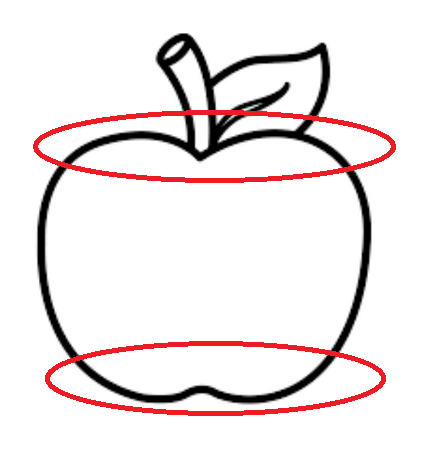
\includegraphics[scale=0.5]{apel}  
	\caption[Bagian pada apel(lingkaran merah) yang akan dibuat menggunakan kurva]{Bagian pada apel(lingkaran merah) yang akan dibuat menggunakan kurva}
	\label{fig:apel} 
\end{figure}

Pertama, tentukan besar apel yang ingin dibuat. Dalam permainan ini besar apel yang dibuat adalah 20 \textit{pixel}. Besar apel dibuat lebih besar dari lebar ular karena jika besar apel sama dengan lebar ular, besar apel terlihat kecil. Selain itu, apel ini digambar pada \textit{layout} yang berbentuk persegi. \textit{Layout} persegi ini juga dapat mempermudah penggambaran apel. Karena menggunakan \textit{layout} persegi, maka \textit{origin} terletak pada titik sudut di sebelah kiri atas. Setelah itu, gambar setiap bagian apel. Bagian apel dibagi menjadi 4 seperti pada Gambar~\ref{fig:apel2} sehingga besar setiap bagian apel tersebut adalah 10 \textit{pixel}. 

\begin{figure}[H]
	\centering  
	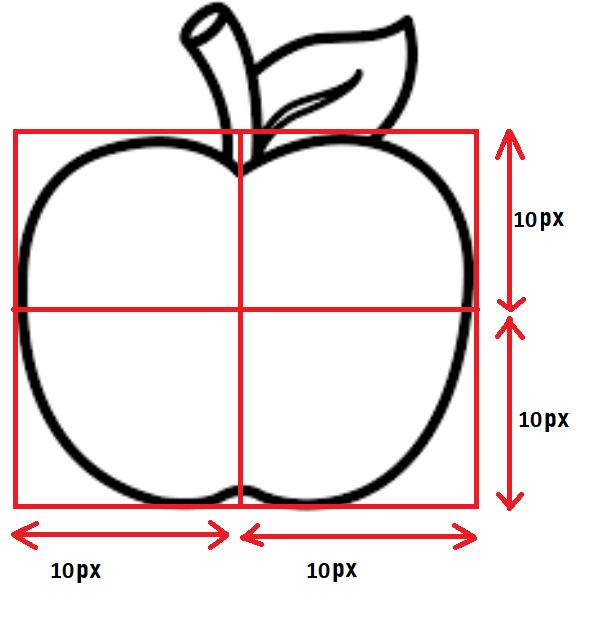
\includegraphics[scale=0.4]{apel2}  
	\caption[Pembagian gambar apel dengan layout persegi beserta ukuran pada setiap bagian]{Pembagian gambar apel dengan layout persegi beserta ukuran pada setiap bagian}
	\label{fig:apel2} 
\end{figure}

Gambar bagian atas apel terlebih dahulu. Gunakan \textit{method moveTo()} untuk menentukan titik mulainya. Titik mulainya terletak pada bagian tengah atas apel yang melengkung ke dalam. Dari titik itu, buat kurva yang \textit{control point}nya adalah titik ujung \textit{layout} persegi. Jika ingin menggambar bagian kiri apel terlebih dahulu maka \textit{control point}nya adalah titik ujung kiri \textit{layout} tersebut. Setelah itu, tentukan \textit{end point} kurva tersebut. Pada Gambar~\ref{fig:apel3} terdapat \textit{start point}, \textit{control point} dan \textit{end point} untuk membuat bagian sisi kiri atas apel. Sesudah itu, buatlah bagian bawah apel. Caranya sama seperti sebelumnya namun \textit{control point}nya dan \textit{end point}nya berbeda. Posisi \textit{control point}nya sedikit menjorok ke dalam dan posisi end pointnya terdapat di tengah bawah seperti pada Gambar~\ref{fig:apel4}. \textit{Start point} tidak perlu diatur lagi, karena \textit{start point}nya sudah tergantikan dengan posisi \textit{end point} pada kurva sebelumnya. Sampai pada bagian ini, bagian kiri apel sudah selesai dibuat. Untuk membuat bagian kanan apel, caranya sama seperti membuat bagian kiri apel. Karena bagian kiri apel simetris dengan bagian kanan apel, maka hanya perlu mengubah \textit{control point} dan \textit{end pointnya} saja. Dengan memanfaatkan bentuk simetris dari apel, maka jarak antara \textit{control point} dan \textit{end point} pada bagian kiri apel dengan batasan tengah sama dengan jarak antara \textit{control point} dan \textit{end point} dengan batas tengah pada bagian kanan apel. 

\begin{figure}[H]
	\centering  
	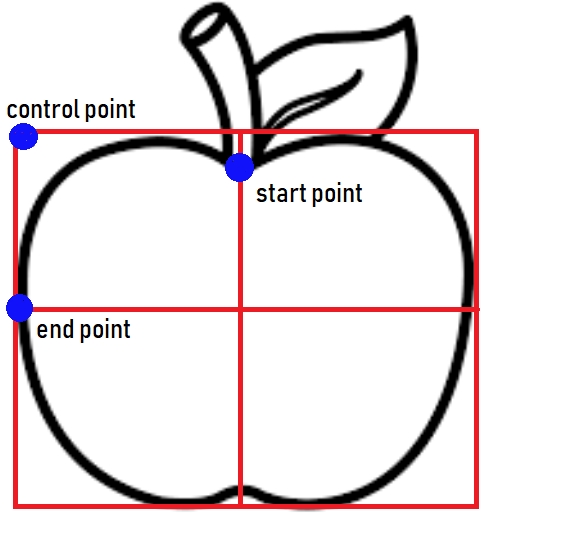
\includegraphics[scale=0.4]{apel3}  
	\caption[\textit{Start point}, \textit{control point} dan \textit{end point} untuk menggambar apel bagian kiri atas]{\textit{Start point}, \textit{control point} dan \textit{end point} untuk menggambar apel bagian kiri atas}
	\label{fig:apel3} 
\end{figure}

\begin{figure}[H]
	\centering  
	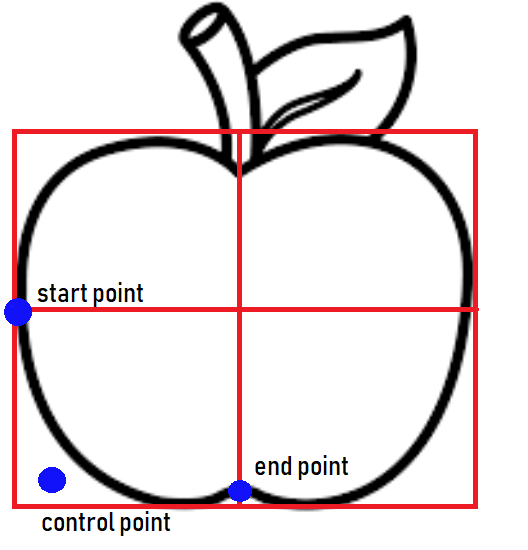
\includegraphics[scale=0.4]{apel4}  
	\caption[\textit{Start point}, \textit{control point} dan \textit{end point} untuk menggambar apel bagian kiri bawah]{\textit{Start point}, \textit{control point} dan \textit{end point} untuk menggambar apel bagian kiri bawah}
	\label{fig:apel4} 
\end{figure}

\subsection{Pergerakan Ular}
Untuk membuat ular bergerak maju, dilakukan penambahan kepala dan pembuangan ekor secara bersamaan ketika ular sedang bergerak maju. Ilustrasinya dapat dilihat pada Gambar~\ref{fig:snakeMoveForward}. Untuk membuat ular bergerak sesuai ilustrasi pada Gambar~\ref{fig:snakeMoveForward}, algoritmanya adalah sebagai berikut : Pertama, semua elemen \textit{array} akan di\textit{shift}/digeser dan elemen pertama akan digantikan dengan koordinat yang baru. Koordinat yang baru tersebut merupakan kepala ular. Setelah itu dilakukan pengecekan apakah panjang tubuh ular lebih besar dari jumlah elemen \textit{array} tubuh ular. Jika benar, maka tidak dilakukan pembuangan elemen terakhir dan jika salah, maka tidak akan dilakukan apa-apa. 

\begin{figure}[H]
	\centering  
	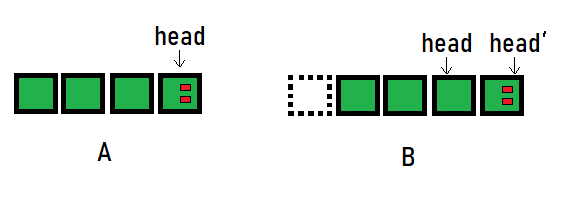
\includegraphics[scale=0.5]{snakeMoveForward}  
	\caption[Ilustrasi ular sebelum bergerak maju(A) dan setelah bergerak maju(B)]{Ilustrasi ular sebelum bergerak maju(A) dan setelah bergerak maju(B)}
	\label{fig:snakeMoveForward} 
\end{figure}

Kecepatan ular pada permainan ini adalah 2,4,6,8 dan 10 \textit{pixel per frame}. Kecepatan ular minimal adalah 1 dan maksimum adalah 5. Kecepatan maksimal ular tidak boleh melebihi lebar tubuh ular. Jika kecepatanya melebihi lebar ular, maka ketika terjadi tabrakan dengan tubuhnya sendiri, kepala ular tidak akan bertabrakan dengan tubuhnya. Kepala ular akan terlihat seolah-olah melompati tubuhnya sendiri. Kecepatan ular tersebut bergantung pada besar bagian tubuh ular karena pada proses penggambaran tubuh ular, bagian koordinat kepala ular akan digeser posisinya di array apabila ular bergerak maju. Misal, jika besar bagian tubuh ular adalah 2 \textit{pixel} dan kecepatan ular adalah 3 \textit{pixel} per \textit{frame}, maka akan ada bagian tubuh ular yang panjangnya 3 \textit{pixel}. Bila diteruskan, maka besar bagian tubuh ular akan menjadi 3. Cara untuk menangani hal ini adalah dengan mengulangi pergerakan ular tersebut sebanyak kecepatan kali. Misal jika besar bagian tubuh ular adalah 2, dan kecepatanya 3, maka ular akan maju sebesar 2 \textit{pixel} sebanyak 3 kali. Kecepatan ular akan menjadi 6 \textit{pixel} per \textit{frame}. Setelah bergerak sebanyak 3 kali, ular akan digambar. Jadi, kecepatan ular merupakan kelipatan dari bagian tubuh ular. \\

Ular dapat berbelok dengan menggunakan tombol pada \textit{keyboard} untuk \textit{desktop} dan menyentuh layar untuk smartphone. Tombol ke kiri dan menekan layar bagian kiri akan membuat ular bergerak melawan arah jarum jam serta tombol ke kanan dan menekan layar bagian kanan akan membuat ular akan bergerak searah jarum jam. Pada permainan yang akan dibuat ini, digunakan sudut sebagai nilai untuk membuat ular dapat bergerak 360$^\circ$. Jika ular bergerak berlawanan arah jarum jam, maka sudut akan berkurang dan jika ular bergerak searah jarum jam, maka sudut akan bertambah. Ketika menambahkan dan mengurangi sudut, perlu dilakukan pengecekan apabila nilai sudut valid atau tidak. Karena nilai sudut yang valid adalah antara nilai 0 sampai 360, maka apabila nilai sudut kurang dari 0, sudut tersebut akan diubah menjadi 360 dan apabila nilai sudut lebih besar dari 360, sudut tersebut akan diubah menjadi 0. Dibutuhkan rumus trigonometri untuk menentukan posisi kepala ular. Untuk menghitung posisi koordinat x pada sudut tertentu, digunakan \textit{cosinus} sedangkan untuk menghitung posisi koordinat y pada sudut tertentu menggunakan \textit{sinus}. Jadi, koordinat x dari kepala ular akan ditambahkan dengan hasil perhitungan cosinus dari sudut dan koordinat y dari kepala ular akan ditambahkan dengan hasil perhitungan sinus dari sudut.

\subsection{Mengacak posisi apel}
Posisi apel akan diacak di daerah \textit{canvas}. Untuk mengacak posisi apel, digunakan fungsi \textit{Math.random()}. Nilai yang akan diacak adalah posisi x dan y dari apel. Hasil dari fungsi \textit{Math.random()} akan dikalikan dengan lebar \textit{canvas} untuk mendapatkan nilai x dan dikalikan dengan tinggi \textit{canvas} untuk mendapatkan nilai y. Karena apel ini dibuat dengan menggunakan \textit{layout} persegi, maka posisi x dan y pada apel terletak di titik sudut kiri atas. Hal ini akan memungkinkan gambar apel akan terpotong seperti yang terlihat pada Gambar~\ref{fig:apelTerpotong}. Misal, besar \textit{canvas} adalah 500 x 500 dan besar apel adalah 10 dan mendapatkan posisi apel adalah (495,10). Posisi x apel ditambah dengan besar apel hasilnya akan melebihi besar \textit{canvas} sehingga membuat sebagian gambar apel terlihat terpotong. Maka dari itu, lebar dan tinggi \textit{canvas} yang dikalikan dengan bilangan acak, akan dikurangi sebesar ukuran apel tersebut.  Nilai yang dihasilkan adalah nilai yang bertipe \textit{float} sedangkan posisi x dan y pada apel membutuhkan \textit{input} bilangan bulat. Untuk mendapatkan bilangan bulat tersebut, nilai yang sudah dihitung tadi dibulatkan ke bawah. Mengacak posisi apel tidak hanya mengacak posisi pada canvas saja, tetapi harus mengecek apakah posisi apel tersebut tidak bertabrakan dengan tubuh ular atau dinding labirin. 

\begin{figure}[H]
	\centering  
	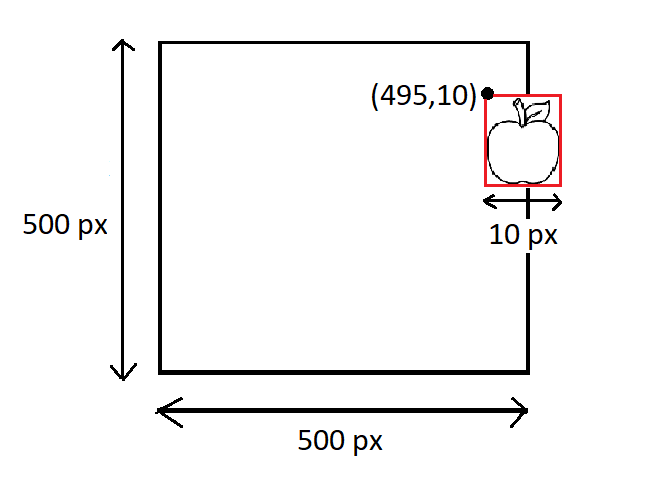
\includegraphics[scale=0.5]{apelTerpotong}  
	\caption[Gambar apel yang terpotong sesudah mengacak posisi apel]{Gambar apel yang terpotong sesudah mengacak posisi apel}
	\label{fig:apelTerpotong} 
\end{figure}

\subsection{Menentukan Besar \textit{Canvas}}
Pada Open Source Snake 360 ini, pemain dapat memainkan permainan tersebut di browser \textit{smartphone} dan \textit{browser desktop}. Hal ini akan memunculkan sebuah kesulitan yaitu menentukan dimensi \textit{canvas} yang cocok bila permainan tersebut dapat dimainkan pada \textit{smartphone} dan \textit{browser} pada \textit{desktop}. Jika disesuaikan dengan layar \textit{desktop}, maka besar \textit{canvas} akan terlihat lebih lebar dibandingkan dengan besar layar pada \textit{smartphone} dan sebaliknya. Cara ini dapat ditangani dengan membuat \textit{canvas} mengikuti besar layar \textit{browser desktop} dan layar \textit{browser smartphone}. Namun, cara ini juga dapat menimbulkan masalah yaitu dalam pembuatan labirin. Format labirin akan terus diubah sesuai dengan besar layar. Untuk menyesuaikan \textit{canvas} dengan besar layar, maka akan dibuat \textit{canvas} berbentuk persegi dengan dimensi $600 \times 600$ \textit{pixel}. Dimensi ini sesuai jika permainan ini dimainkan pada \textit{smartphone} dan \textit{desktop}. Selain menentukan dimensi, besar objek yang ada pada canvas juga harus diperbesar agar objek-objek pada \textit{canvas} tidak terlihat kecil bagi pemain bermain menggunakan \textit{smartphone}. 

\subsection{Menggambar Labirin}
Pada permainan ini, format labirin dapat dibuat dengan menggunakan JSON dan \textit{file} teks. Permainan ini menggunakan \textit{file} teks sebagai format labirin, karena \textit{file} text lebih mudah untuk dibuat dan dimengerti oleh pembuat labirin. Labirin dibuat menggunakan simbol '\#' dan '-'. Setiap simbol merepresentasikan besar dinding. Daerah yang merupakan dinding labirin ditulis dengan menggunakan simbol '\#' sedangkan untuk daerah yang bukan merupakan dinding labirin ditulis dengan menggunakan simbol '-'. Jika pada \textit{file} tersebut terdapat teks '\#-\#', itu artinya menggambar dinding, tidak menggambar dinding dan menggambar dinding lagi. Hasilnya dapat dilihat pada Gambar~\ref{fig:gambarDinding}. Besar \textit{canvas} untuk permainan ini adalah $600 \times 600$ \textit{pixel} dan besar dinding labirin sebesar 10 \textit{pixel}. Besar dinding tidak boleh lebih kecil dari lebar tubuh ular. Apabila besar dinding lebih kecil dari ular, ular tidak akan dapat melewati jalur yang diapit oleh 2 buah dinding seperti yang terlihat pada Gambar~\ref{fig:ularDinding}. Jumlah baris pada \textit{file} teks akan disamakan dengan jumlah kolomnya. Sesuai dengan besar \textit{canvas} dan besar dinding labirin yaitu $600 \times 600$ \textit{pixel}, maka dapat ditentukan bahwa setiap \textit{file} teks memiliki 60 baris dan setiap barisnya terdiri dari 60 karakter. Untuk menggambar dinding secara horizontal, maka hanya menggambar garis dengan panjang 10 \textit{pixel} dari titik awal ke titik akhir. Sebagai contoh, apabila karakter pada baris pertama dan kolom pertama adalah '\#', maka dinding akan digambar pada \textit{canvas} dari titik(0,0) sampai titik(10,0) dengan lebar dinding 10 pixel. \textit{Level} pada labirin dapat ditentukan berdasarkan kerumitan labirin. Labirin yang memiliki dinding yang banyak dan kompleks akan mendapatkan \textit{level} yang lebih tinggi dibandingkan dengan labirin yang memiliki sedikit dinding dan lebih simpel. \\

Untuk mendapatkan \textit{file} labirin, \textit{Javascript} tidak dapat digunakan karena \textit{Javascript} tidak dapat membaca \textit{file} dari server. Oleh karena itu, AJAX akan digunakan untuk membaca isi labirin dari \textit{folder}. Dengan menggunakan AJAX, terdapat sebuah masalah yaitu AJAX bersifat \textit{asynchronous} yang menyebabkan labirin belum selesai digambar sebelum permainan sudah siap untuk dimainkan. Cara untuk menangani masalah ini adalah dengan menggunakan \textit{callback}. Dengan adanya \textit{callback}, dapat dipastikan bahwa permainan sudah siap untuk dimainkan apabila labirin sudah selesai digambar.\\ 

\begin{figure}[H]
	\centering  
	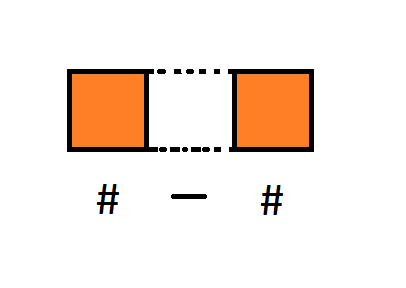
\includegraphics[scale=0.5]{gambarDinding}  
	\caption[Menggambar dinding menggunakan simbol pada file teks]{Menggambar dinding menggunakan simbol pada file teks}
	\label{fig:gambarDinding} 
\end{figure}

\begin{figure}[H]
	\centering  
	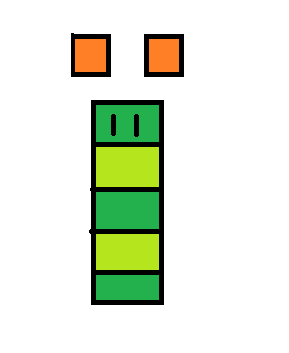
\includegraphics[scale=0.5]{ularDinding}  
	\caption[Ular ingin melewati jalur yang diapit oleh 2 buah dinding]{Ular ingin melewati jalur yang diapit oleh 2 buah dinding}
	\label{fig:ularDinding} 
\end{figure}

\subsection{Pengecekan tabrakan(\textit{Collision Detection})}
Pada permainan ini terdapat pengecekan tabrakan yang dapat mengecek apakah ular sudah memakan makanan, ular menabrak tubuhnya sendiri, dan ular menabrak dinding labirin. Seluruh pengecekan ini akan dilakukan pada setiap \textit{frame}. Pada pengecekan tabrakan pada apel dan ular, hanya perlu mengecek tabrakan antara kepala ular dengan apel. Karena jalur yang dilalui oleh kepala ular, akan selalu dilalui oleh bagian tubuh ular. Dengan kata lain, bagian tubuh ular akan mengikuti ke mana kepala ular akan bergerak. Dengan ini, tidak perlu dilakukan \textit{collision detection} antara bagian tubuh ular dengan apel. Untuk mengetahui terjadinya tabrakan antara ular dengan apel, maka akan dibuat daerah tabrakan pada apel. Daerah tabrakan ini digunakan untuk mengecek apakah 2 benda saling bertabrakan satu sama lain. Daerah tabrakan pada apel ditandai dengan arsiran bewarna merah yang terdapat pada Gambar~\ref{fig:apelArsir}. Namun, untuk membuat daerah tabrakan ini cukup sulit ketika mengecek adanya tabrakan antara ular dengan apel terutama pada bagian lengkungan pada apel. Karena itu, daerah tabrakan pada apel dibuat dengan menggunakan bentuk persegi seperti pada Gambar~\ref{fig:apelArsirPersegi}. Jika posisi kepala ular berada di dalam daerah tabrakan apel, maka dapat dipastikan bahwa ular tersebut sudah memakan apel.\\

\begin{figure}[H]
	\centering  
	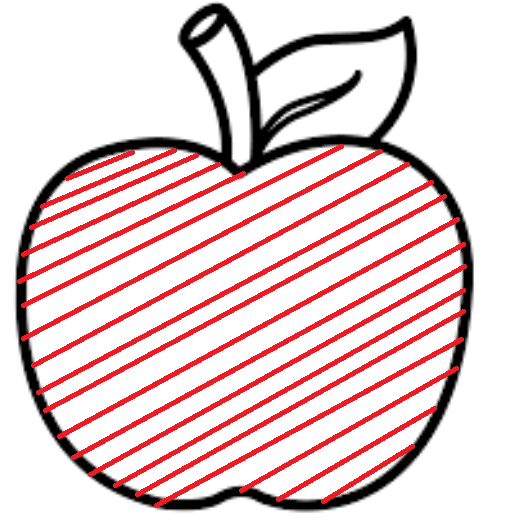
\includegraphics[scale=0.4]{apelArsir}  
	\caption[Daerah tabrakan pada apel]{Daerah tabrakan pada apel}
	\label{fig:apelArsir} 
\end{figure}

\begin{figure}[H]
	\centering  
	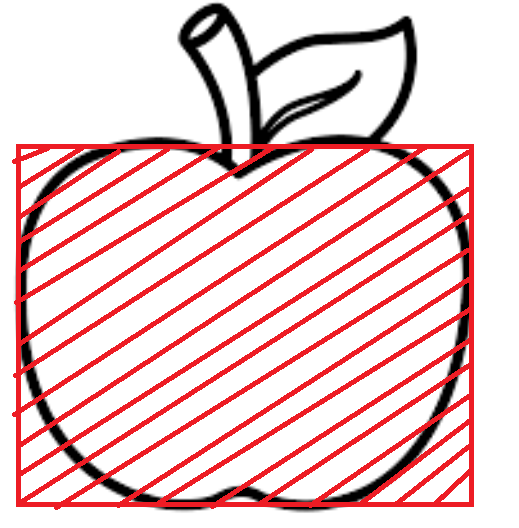
\includegraphics[scale=0.4]{apelArsirPersegi}  
	\caption[Daerah tabrakan berbentuk persegi pada apel]{Daerah tabrakan berbentuk persegi pada apel}
	\label{fig:apelArsirPersegi} 
\end{figure}

Untuk mengecek tabrakan antara ular dengan tubuhnya sendiri adalah dengan mengecek tabrakan antara kepala ular dengan seluruh bagian tubuh ular. Ular dapat dipastikan menabrak tubuhnya sendiri apabila ketentuan berikut telah terpenuhi : 

\begin{itemize}
	\item koordinat x kepala ular lebih kecil dari koordinat x bagian tubuh ular dikurangi panjang bagian tubuh ular
	\item koordinat x kepala ular lebih besar dari koordinat x bagian tubuh ular ditambah dengan panjang bagian tubuh ular
	\item koordinat y kepala ular lebih kecil dari koordinat y bagian tubuh ular dikurangi panjang bagian tubuh ular
	\item koordinat y kepala ular lebih besar dari koordinat y bagian tubuh ular ditambah dengan panjang bagian tubuh ular
\end{itemize}

Untuk mengecek tabrakan dengan dinding labirin, dilakukan pengecekan antara kepala ular dengan sebuah dinding. Bila dilakukan pengecekan antara kepala ular dengan seluruh dinding labirin, maka animasi permainan akan berjalan lebih lambat. Semakin banyak dinding, animasi akan berjalan lebih lambat. Cara untuk mengecek tabrakan antara kepala ular dengan dinding adalah sebagai berikut : misal posisi kepala ular adalah (9,13). Jika besar dinding adalah 10 pixel, maka kepala ular akan berada di daerah pada koordinat (0,10) sampai (10,20). Pada Gambar~\ref{fig:posisiPadaDinding} terdapat gambaran untuk memperjelas contoh tersebut. Kemudian, posisi kepala ular tersebut akan dibagi dengan besar dinding (10 pixel). Hasil yang didapat dari perhitungan tersebut adalah (0,1). Hasil tersebut akan digunakan untuk mengecek dinding pada labirin yang diambil dari file teks yang sudah disimpan di \textit{array}. Karena hasil dari perhitungan tersebut adalah (0,1) maka akan dicek apakah array elemen kedua dan karakter pertama merupakan dinding. Misal pada array elemen kedua dan karakter pertama merupakan dinding, maka kepala ular menabrak dinding.

\begin{figure}[H]
	\centering  
	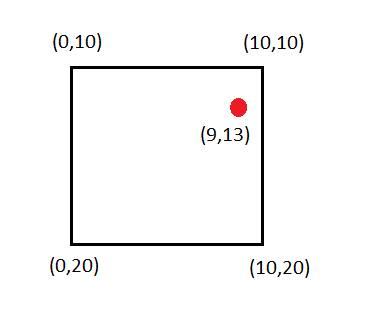
\includegraphics[scale=0.5]{posisiPadaDinding}  
	\caption[Posisi kepala ular pada sebuah daerah labirin]{Posisi kepala ular pada sebuah daerah labirin}
	\label{fig:posisiPadaDinding} 
\end{figure}

\section{Analisis Berorientasi Objek}

\subsection{Skenario Permainan}
Pada bagian ini akan dijelaskan dan ditunjukkan diagram \textit{use case} dari permainan \textit{Snake} 360. Penjelasan meliputi skenario, aktor, prakondisi skenario normal dan eksepsi. Aktor yang melakukanya adalah pemain. Pada Gambar~\ref{fig:useCase} terdapat diagram \textit{use case} dari permainan \textit{Snake} 360.

\begin{figure}[H]
	\centering  
	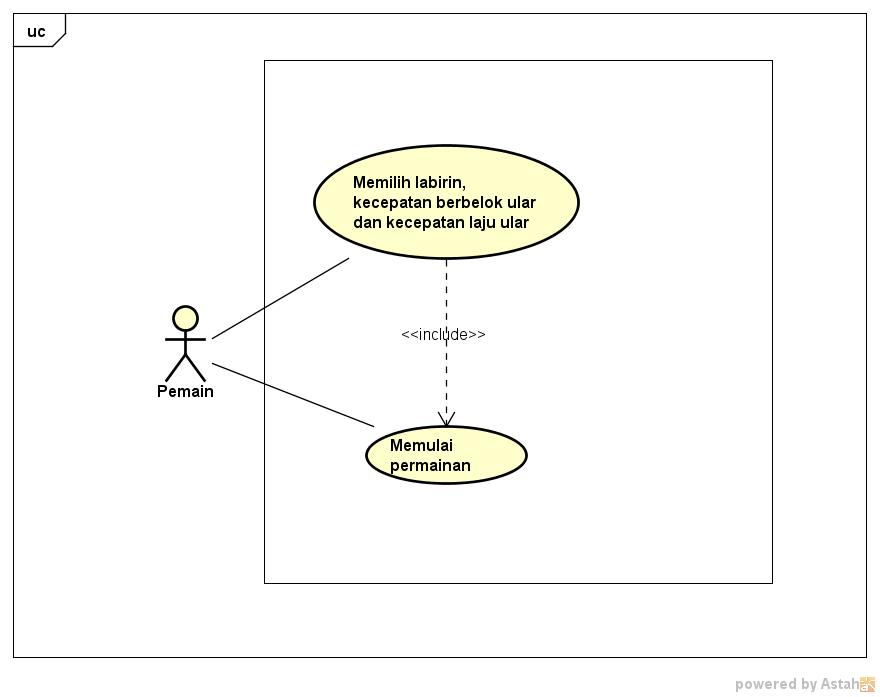
\includegraphics[scale=0.4]{useCase}  
	\caption[Diagram \textit{use case} dari permainan \textit{Snake} 360]{Diagram \textit{use case} dari permainan \textit{Snake} 360}
	\label{fig:useCase} 
\end{figure}

Berikut adalah skenario dari diagram \textit{use case} :

\begin{enumerate}
	\item Skenario : Mulai bermain \\
Aktor : Pemain \\
Prakondisi : Pemain memulai permainan.\\
Skenario normal : Pemain memulai bermain. Setelah memilih, pemain akan memilih level dan labirin. \\
Eksepsi : - \\

	\item Skenario : Memilih level labirin dan kecepatan ular \\
Aktor : Pemain \\
Prakondisi : Pemain sudah mulai bermain. \\
Skenario normal : Pemain memilih level dan labirin yang diinginkan. \\ 
Eksepsi : - \\
\end{enumerate}

\subsection{Diagram Kelas}
Pada Gambar~\ref{fig:classDiagram} terdapat diagram kelas dari \textit{Snake} 360.

\begin{figure}[H]
	\centering  
	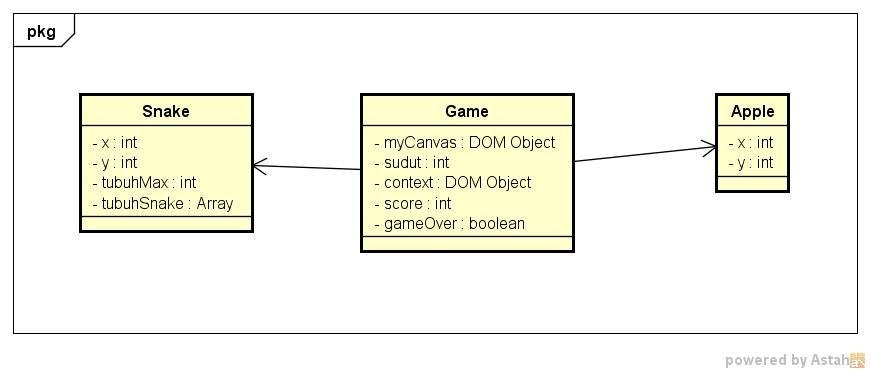
\includegraphics[scale=0.4]{classDiagram}  
	\caption[Diagram class dari permainan \textit{Snake} 360]{Diagram kelas dari permainan \textit{Snake} 360}
	\label{fig:classDiagram} 
\end{figure}

Diagram kelas terdiri dari beberapa kelas yaitu :

\begin{enumerate}
	\item Kelas Snake merupakan  kelas yang merepresentasikan objek ular.
	\item Kelas Apple merupakan kelas yang merepresentasikan objek apel.
	\item Kelas Game merupakan kelas yang mengatur jalanya permainan.
	\item Kelas Maze merupakan kelas yang merepresentasikan objek labirin.
	\item Kelas DrawingObject merupakan kelas untuk menggambar semua objek pada canvas.
\end{enumerate}

Berikut adalah atribut yang dimiliki setiap kelas :

\begin{enumerate}
	\item Kelas Snake\\
\textbf{int}

\begin{itemize}
	\item x, merupakan posisi ular pada koordinat x.
	\item y, merupakan posisi ular pada koordinat y.
	\item tubuhMax, merupakan panjang tubuh ular.
	\item besarUlar, merupakan lebar tubuh ular.
\end{itemize}

\textbf{Array}

\begin{itemize}
	\item tubuhSnake, merupakan posisi tubuh ular pada koordinat x dan y.
\end{itemize}

	\item Kelas Apel\\
	\textbf{int}
	
\begin{itemize}
	\item x, merupakan posisi apel pada koordinat x.
	\item y, merupakan posisi apel pada koordinat y.
	\item besarApel, merupakan besar apel.
\end{itemize}

\item Kelas Game \\
\textbf{int}

\begin{itemize}
	\item sudut, merupakan besar sudut yang digunakan untuk ular berbelok.
	\item score, merupakan skor yang didapat pada permainan.
	\item CANVAS\_SIZE, merupakan lebar dan tinggi canvas.
	\item GRID\_SIZE, merupakan besar grid.
\end{itemize}

\textbf{DOM Object}

\begin{itemize}
	\item myCanvas, merupakan objek \textit{canvas} untuk menggambar ular dan apel.
	\item context, merupakan \textit{context} 2D pada \textit{myCanvas}. 
	\item mazeCanvas, merupakan objek canvas untuk menggambar labirin.
	\item contextMaze, merupakan \textit{context} 2D  pada \textit{mazeCanvas}.
\end{itemize}

\textbf{boolean}
\begin{itemize}
	\item gameOver, memberitahu apakah permainan sudah berakhir atau belum.
\end{itemize}

\item Kelas Maze \\
\textbf{int}

\begin{itemize}
	\item besarDinding, merupakan besar lebar dinding.
\end{itemize}

\textbf{Array}

\begin{itemize}
	\item maze, merupakan layout labirin.
\end{itemize}

\item DrawingObject \\
\textbf{DOM Object}

\begin{itemize}
	\item context, merupakan objek canvas untuk menggambar ular dan apel.
	\item contextMaze, merupakan objek canvas untuk menggambar labirin.
\end{itemize}

\end{enumerate}